\documentclass{article}
\usepackage[T1]{fontenc}
\usepackage{fancyhdr}
\usepackage{extramarks}
\usepackage{amsmath}
\usepackage{amsthm}
\usepackage{amsfonts}
\usepackage{dsfont}
\usepackage{tikz}
\usepackage[plain]{algorithm}
\usepackage{algpseudocode}
\usepackage{graphicx}
\usepackage{listings}
\usepackage{multicol,multirow,array,listings,tabularx,lastpage,textcomp,booktabs}
\usepackage{amssymb}
\usepackage{enumerate}
\usepackage{color}

\usetikzlibrary{automata,positioning,arrows}

\graphicspath{ {./img} } 

\definecolor{light-gray}{gray}{0.95}

\lstset{numbers=right, 
        numberstyle=\tiny, 
        breaklines=true,
        backgroundcolor=\color{light-gray},
        numbersep=5pt,
        xleftmargin=.25in,
        xrightmargin=.25in,
        tabsize=4} 

\lstset{language=C++} 

%
% Basic Document Settings
%

\topmargin=-0.45in
\evensidemargin=0in
\oddsidemargin=0in
\textwidth=6.5in
\textheight=9.0in
\headsep=0.25in

\linespread{1.1}

\pagestyle{fancy}
\lhead{\hmwkAuthorName}
\chead{\hmwkTitle}
\rhead{\hmwkClass}
\lfoot{\lastxmark}
\cfoot{\thepage}

\renewcommand\headrulewidth{0.4pt}
\renewcommand\footrulewidth{0.4pt}

\setlength\parindent{0pt}
\setlength{\parskip}{5pt}

%
% Homework Details
%   - Title
%   - Due date
%   - Class
%   - Section/Time
%   - Instructor
%   - Author
%

\newcommand{\hmwkTitle}{Project Task 1}
\newcommand{\hmwkDueDate}{Feb 22, 2024}
\newcommand{\hmwkClass}{CSE 105}
\newcommand{\hmwkClassInstructor}{Professor Minnes}
\newcommand{\hmwkAuthorName}{\textbf{Ray Tsai}}
\newcommand{\hmwkPID}{A16848188}

%
% Title Page
%

\title{
    \vspace{2in}
    \textmd{\textbf{\hmwkClass:\ \hmwkTitle}}\\
    \normalsize\vspace{0.1in}\small{Due\ on\ \hmwkDueDate\ at 5:00pm}\\
    \vspace{0.1in}\large{\textit{\hmwkClassInstructor}} \\
    \vspace{3in}
}

\author{
  \hmwkAuthorName \\
  \vspace{0.1in}\small\hmwkPID
}
\date{}

%
% Various Helper Commands
%

% Useful for algorithms
\newcommand{\alg}[1]{\textsc{\bfseries \footnotesize #1}}

% For derivatives
\newcommand{\deriv}[1]{\frac{\mathrm{d}}{\mathrm{d}x} (#1)}

% For partial derivatives
\newcommand{\pderiv}[2]{\frac{\partial}{\partial #1} (#2)}

% Integral dx
\newcommand{\dx}{\mathrm{d}x}

% Probability commands: Expectation, Variance, Covariance, Bias
\newcommand{\Var}{\mathrm{Var}}
\newcommand{\Cov}{\mathrm{Cov}}
\newcommand{\Bias}{\mathrm{Bias}}
\newcommand*{\Z}{\mathbb{Z}}
\newcommand*{\Q}{\mathbb{Q}}
\newcommand*{\R}{\mathbb{R}}
\newcommand*{\C}{\mathbb{C}}
\newcommand*{\N}{\mathbb{N}}
\newcommand*{\prob}{\mathds{P}}
\newcommand*{\E}{\mathds{E}}

\begin{document}

\maketitle

\pagebreak

\section*{Introduction}

This documentation outlines a C++ program designed to convert a Non-deterministic Finite Automaton (NFA) into a Deterministic Finite Automaton (DFA). The conversion process preserves the recognized language by following the canonical construction procedure, ensuring that the DFA accepts the same set of strings as the original NFA.

The program operates on NFAs defined over the binary alphabet $\Sigma = \{a, b\}$, representing NFA's and DFA's with the formal definitions. States $Q$ within the NFA are represented as integers, ranging from 0 to $n - 1$, where $n$ is the total number of states. Upon conversion, the program generates a DFA, with its set of states represented as $\mathcal{P}(Q)$, the set of all possible subsets of $Q$.

The transition functions for both the NFA and the resultant DFA are delineated in a tabular format. In these tables, rows correspond to the current states, and columns correspond to the input alphabet symbols. Each cell within the table encapsulates the possible state transitions given a particular input symbol. Despite the transition tables for both the NFA and DFA display cells containing subsets of $Q$, it's important to note that in the NFA, these cells represent sets of possible next states for a given input, while in the DFA, each cell corresponds to a single composite state that encapsulates the possible NFA states after a transition.

\section*{Example}

To illustrate the functionality of the program, we will proceed with the example of NFA $N$ detailed below:

\begin{center}
  State diagram of $N$

  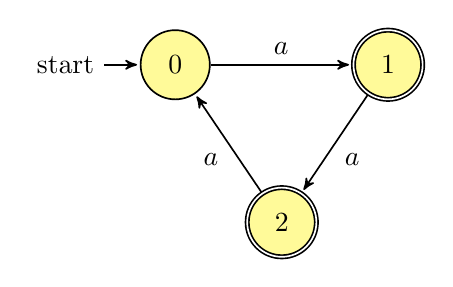
\begin{tikzpicture}[->,>=stealth',shorten >=1pt, auto, node distance=2cm, semithick]
    \tikzstyle{every state}=[text=black, fill=yellow!40]
    
    \node[initial,state] (0)          {$0$}; \node[state, accepting] (1) [right of=0, xshift=20pt] {$1$}; \node[state, accepting] (2) [below of=0, xshift=38.5pt] {$2$};

    \path (0) edge  [] node {$a$} (1) (1) edge  [] node {$a$} (2) (2) edge  [] node {$a$} (0);
    \end{tikzpicture}
\end{center}

$N$ accepts strings over $\Sigma$ that only contain $a$ and have lengths are not divisible by three. In formal terms, $L(N) = \{w \in L(a^*) \mid |w| \nmid 3\}$. For example, $N$ accepts $a$ but rejects $aaa$.

\section*{Instruction}


To begin, we initiate the compilation process by executing the \verb|make| command in the terminal. Once compilation is successfully completed, we run the program with \verb|./compile|. The program will then prompt us to enter the parameters for our NFA, which include the number of states, the start state, the accepting states, and the transition function outputs for each state and symbol pair. Note that when inputting a set of states into the program, the states should be entered in sequence and separated by spaces. For instance, to input the set $\{0, 1, 2\}$, we entered it in the format \verb|0 1 2|. If we were to input $\emptyset$, we may simply click enter.

We now proceed with a step-by-step walkthrough of entering the NFA $N$ into the program. 

\newpage

\textbf{\large Enter the number of states}

Since $N$ contains $3$ states, we enter \verb|3|.

\begin{center}
  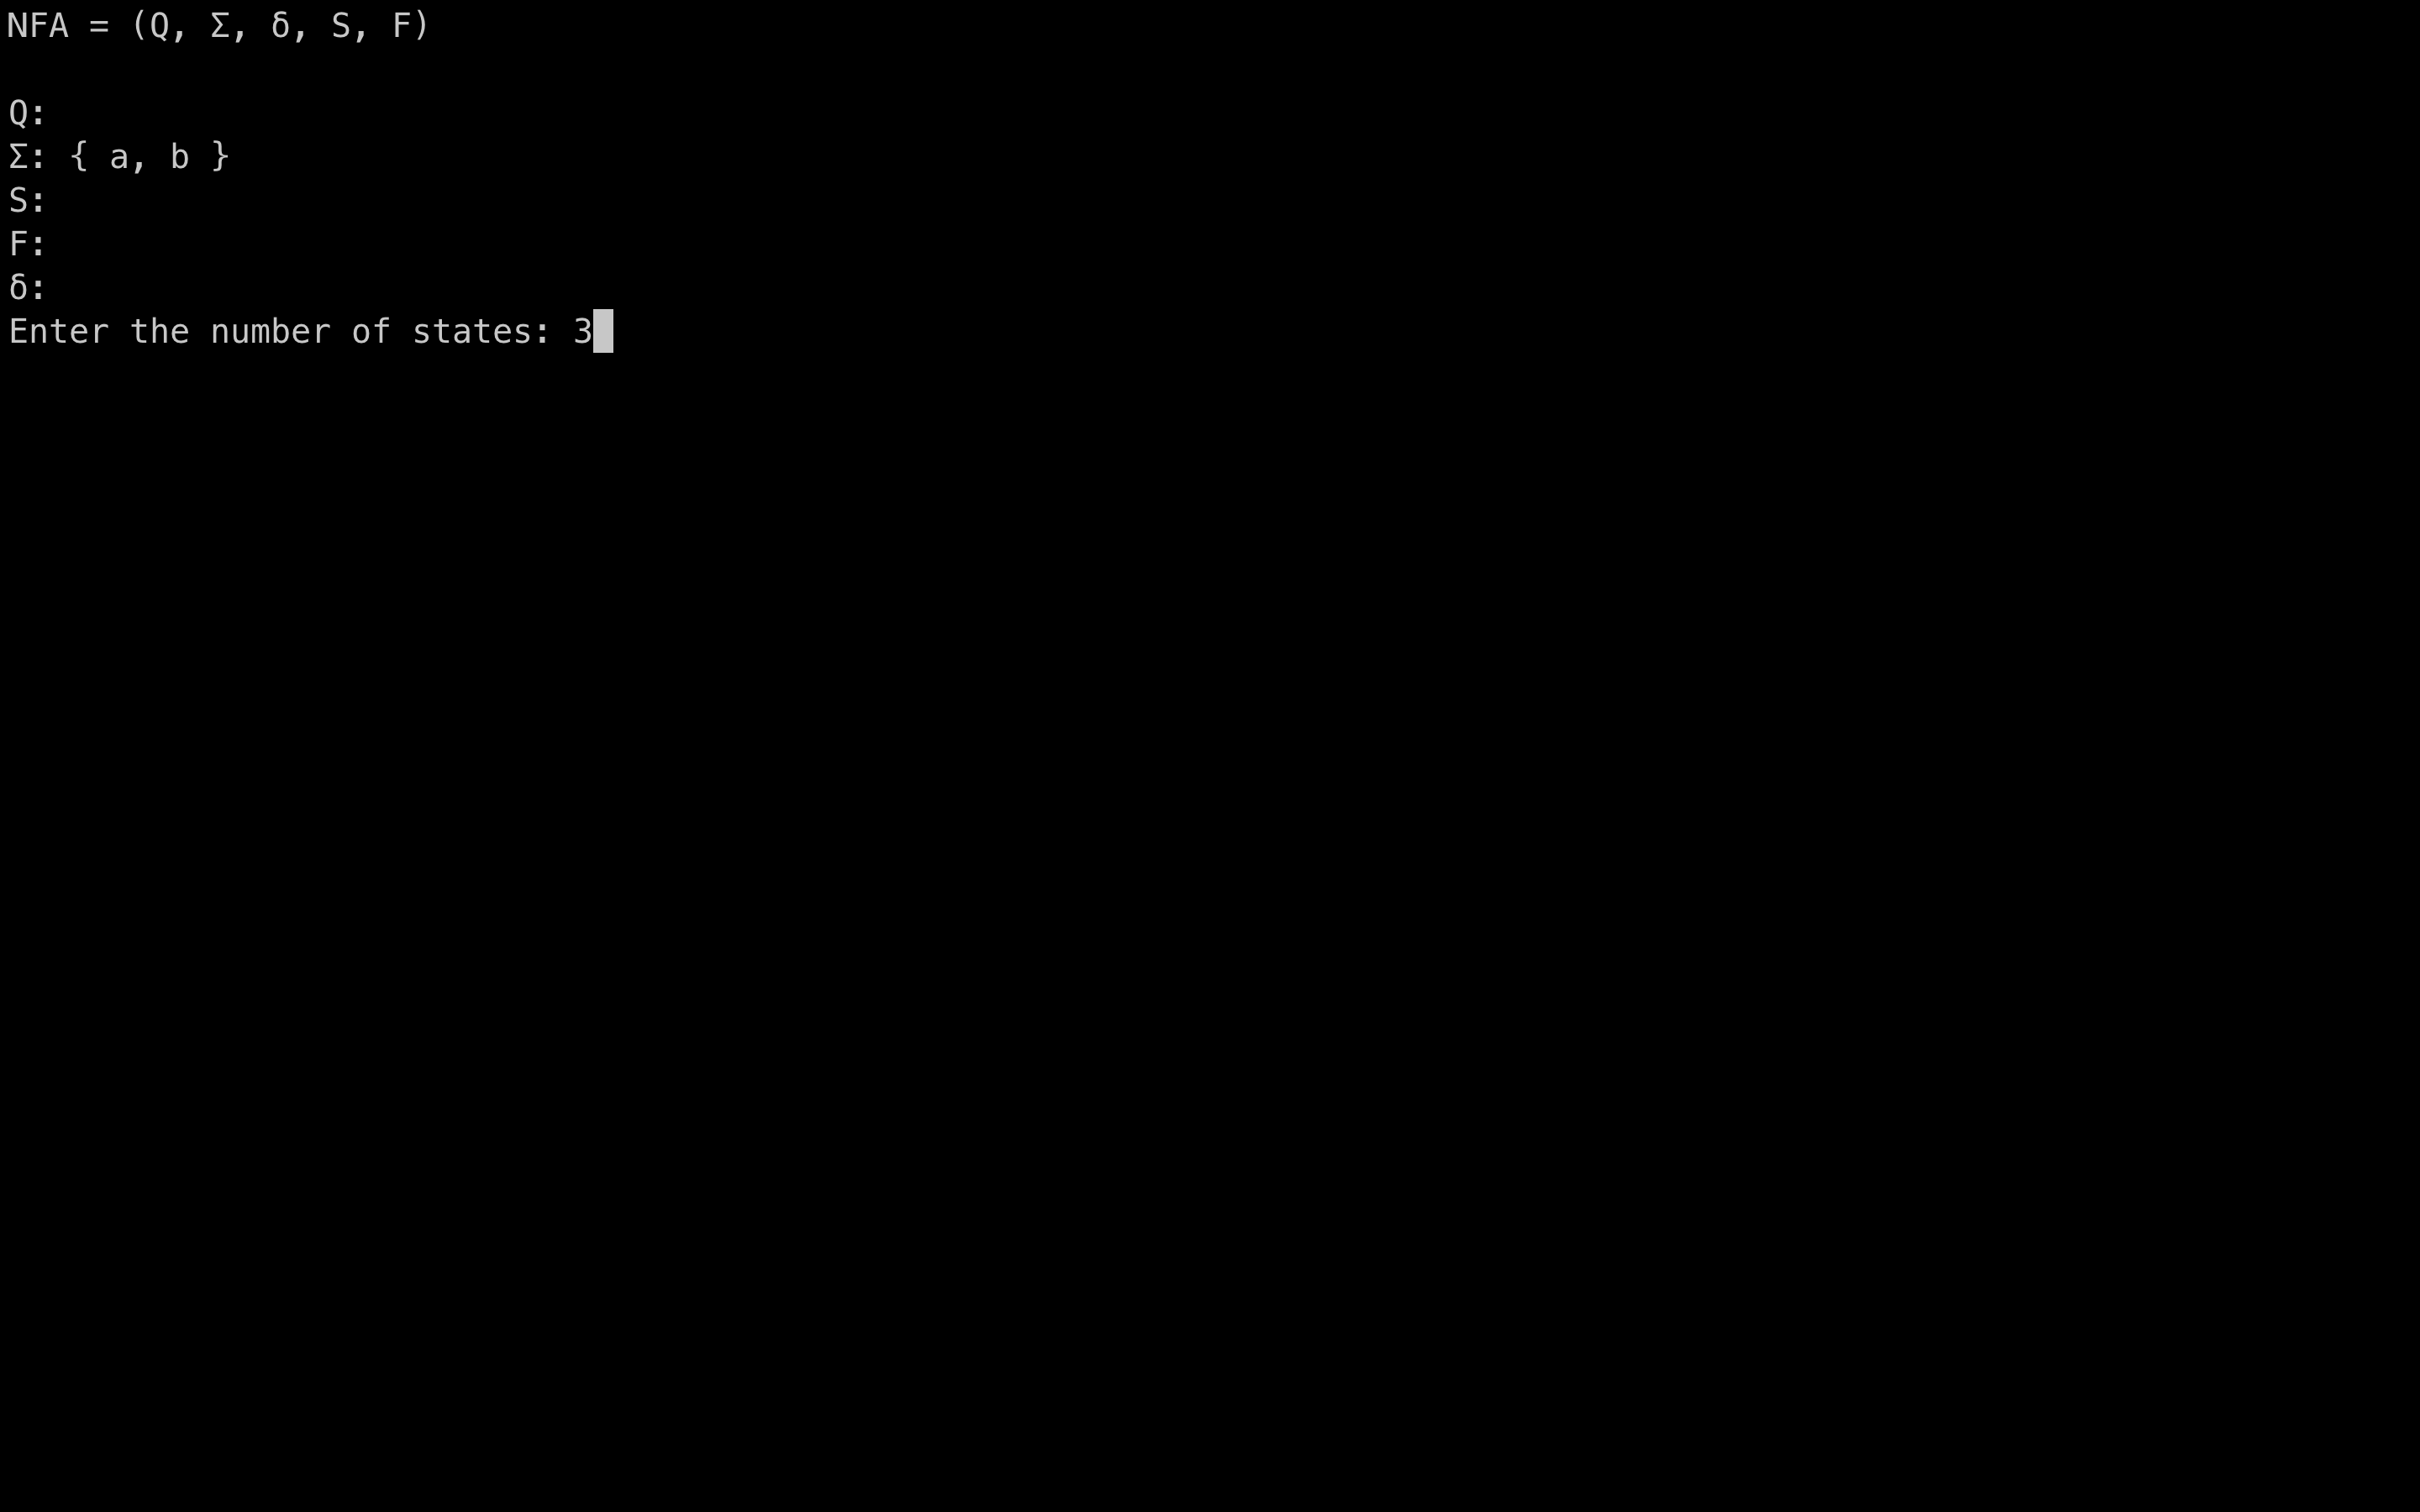
\includegraphics[width=0.8\textwidth]{num}
\end{center}


\textbf{\large Enter the starting state}

We enter \verb|0|, the starting state of $N$.

\begin{center}
  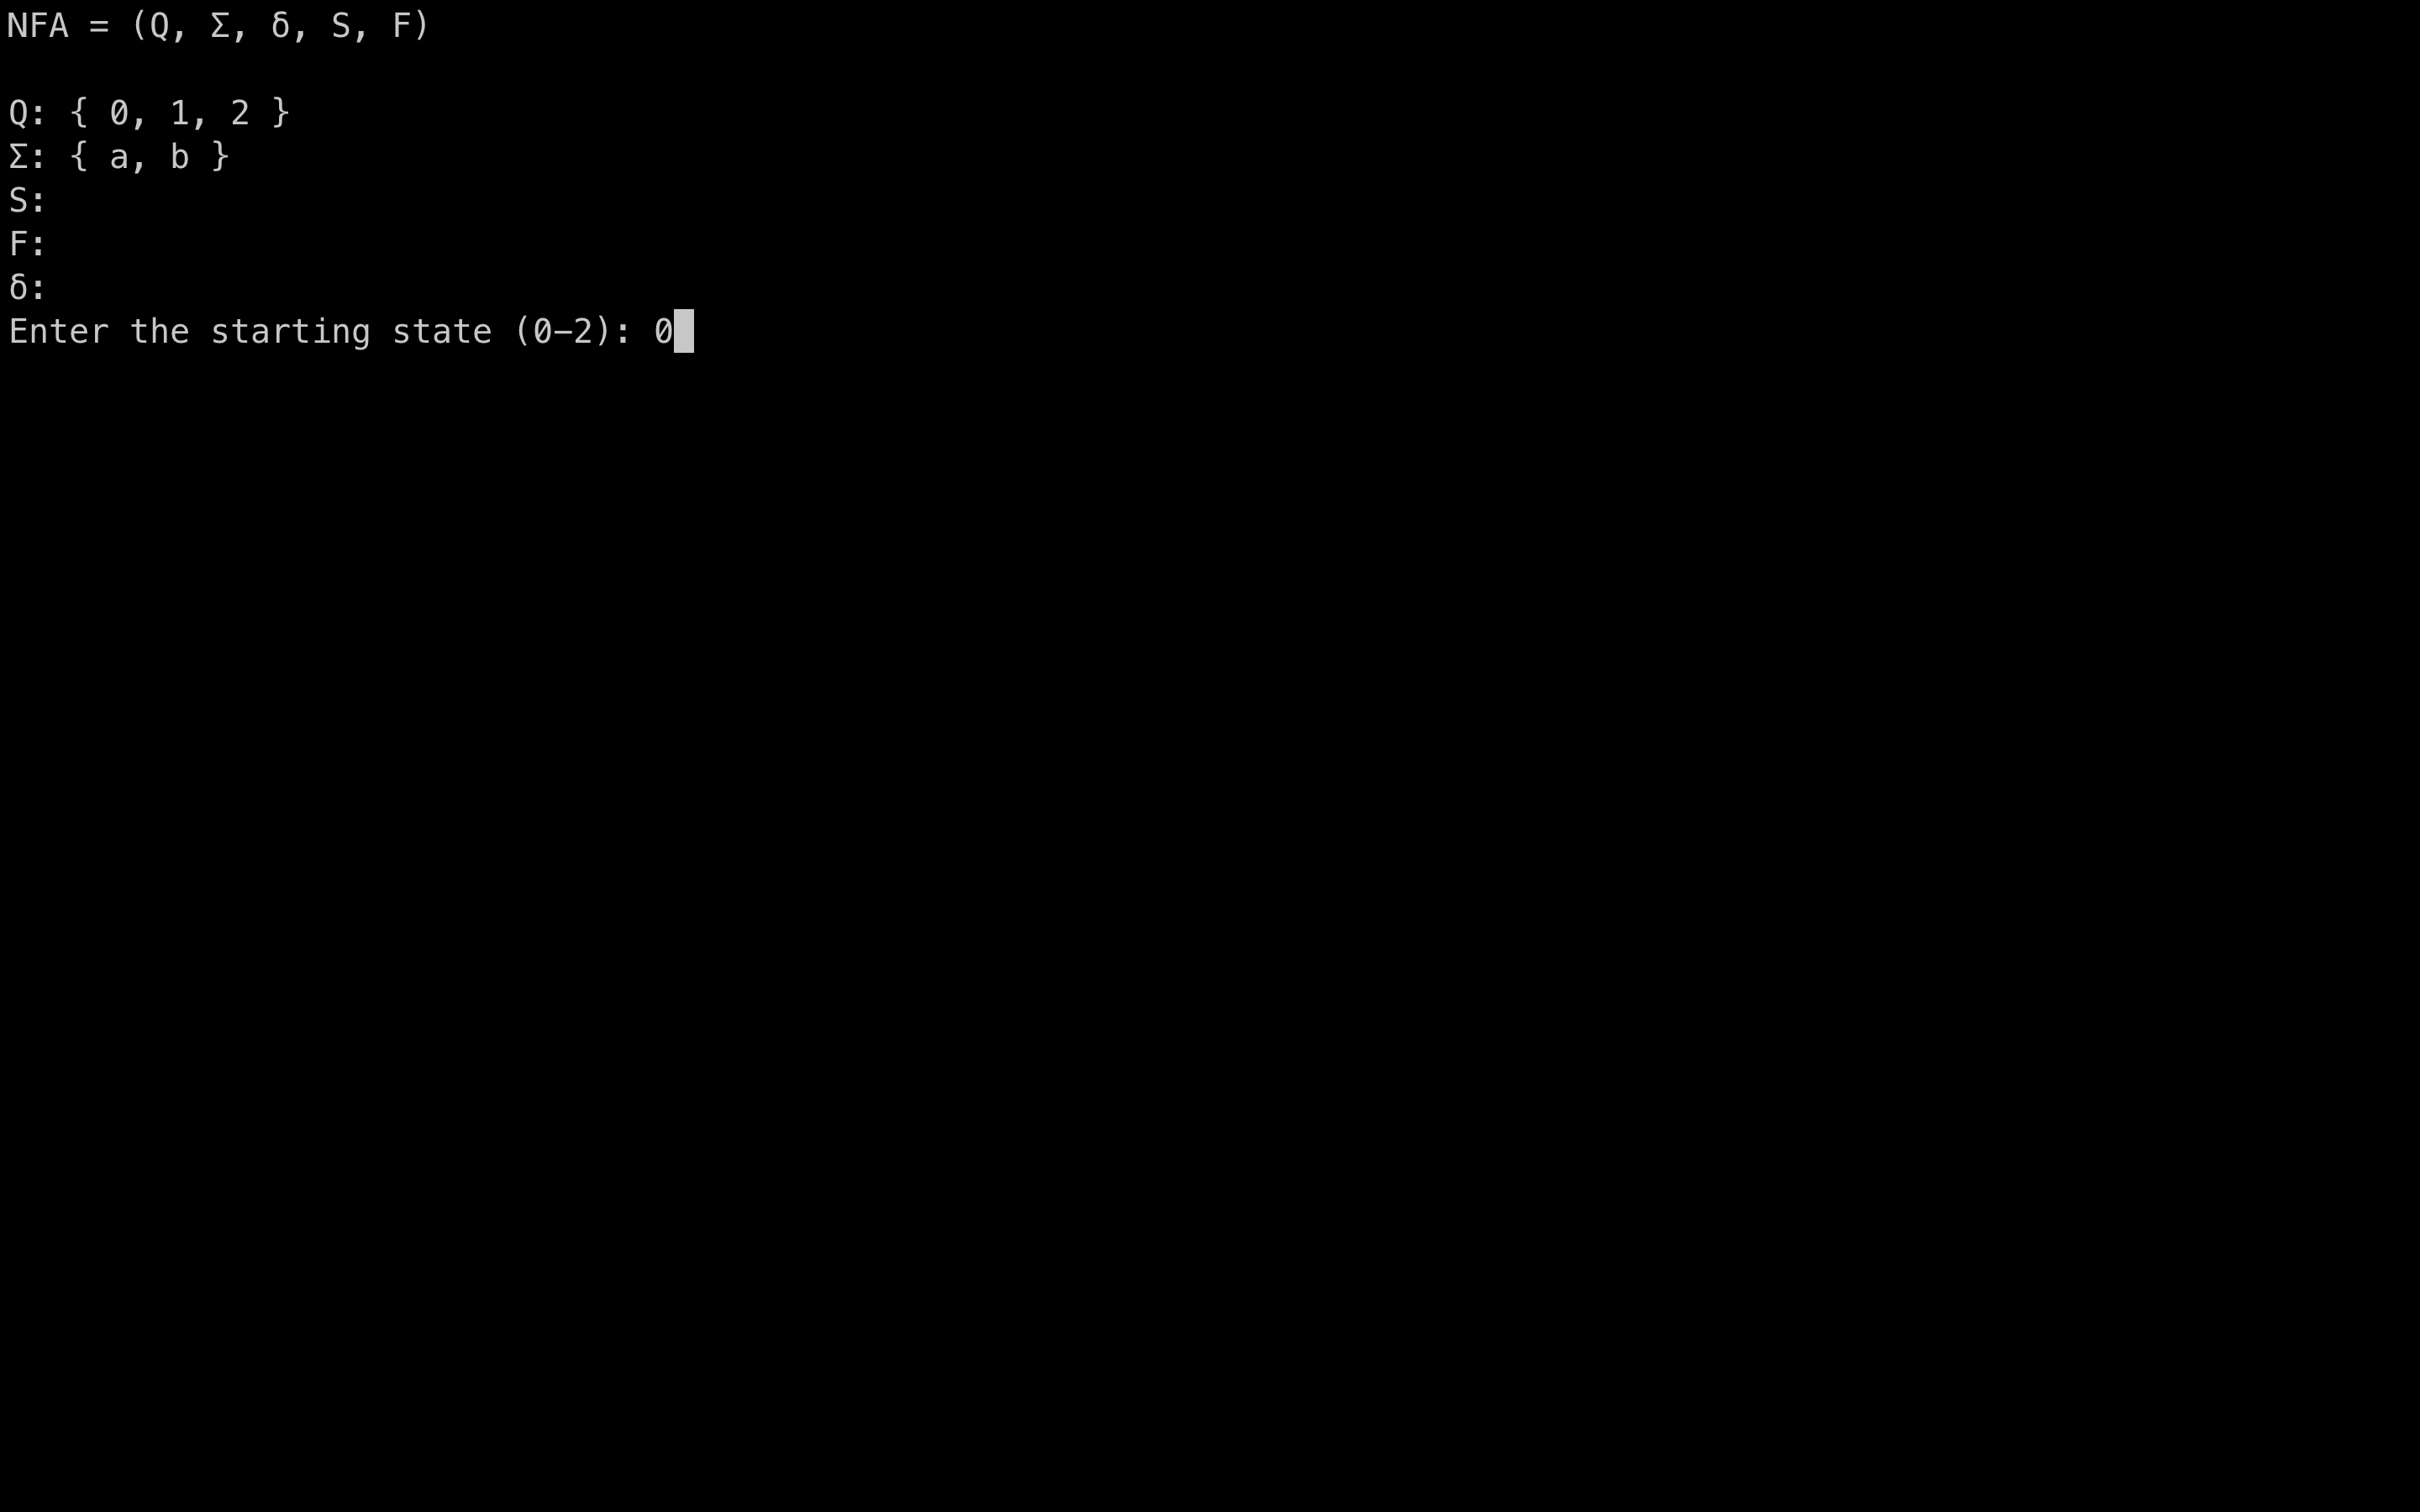
\includegraphics[width=0.8\textwidth]{start}
\end{center}

\newpage

\textbf{\large Enter the accepting states}

We enter the set of accepting states of $N$ in the designated format, which is \verb|1 2|.

\begin{center}
  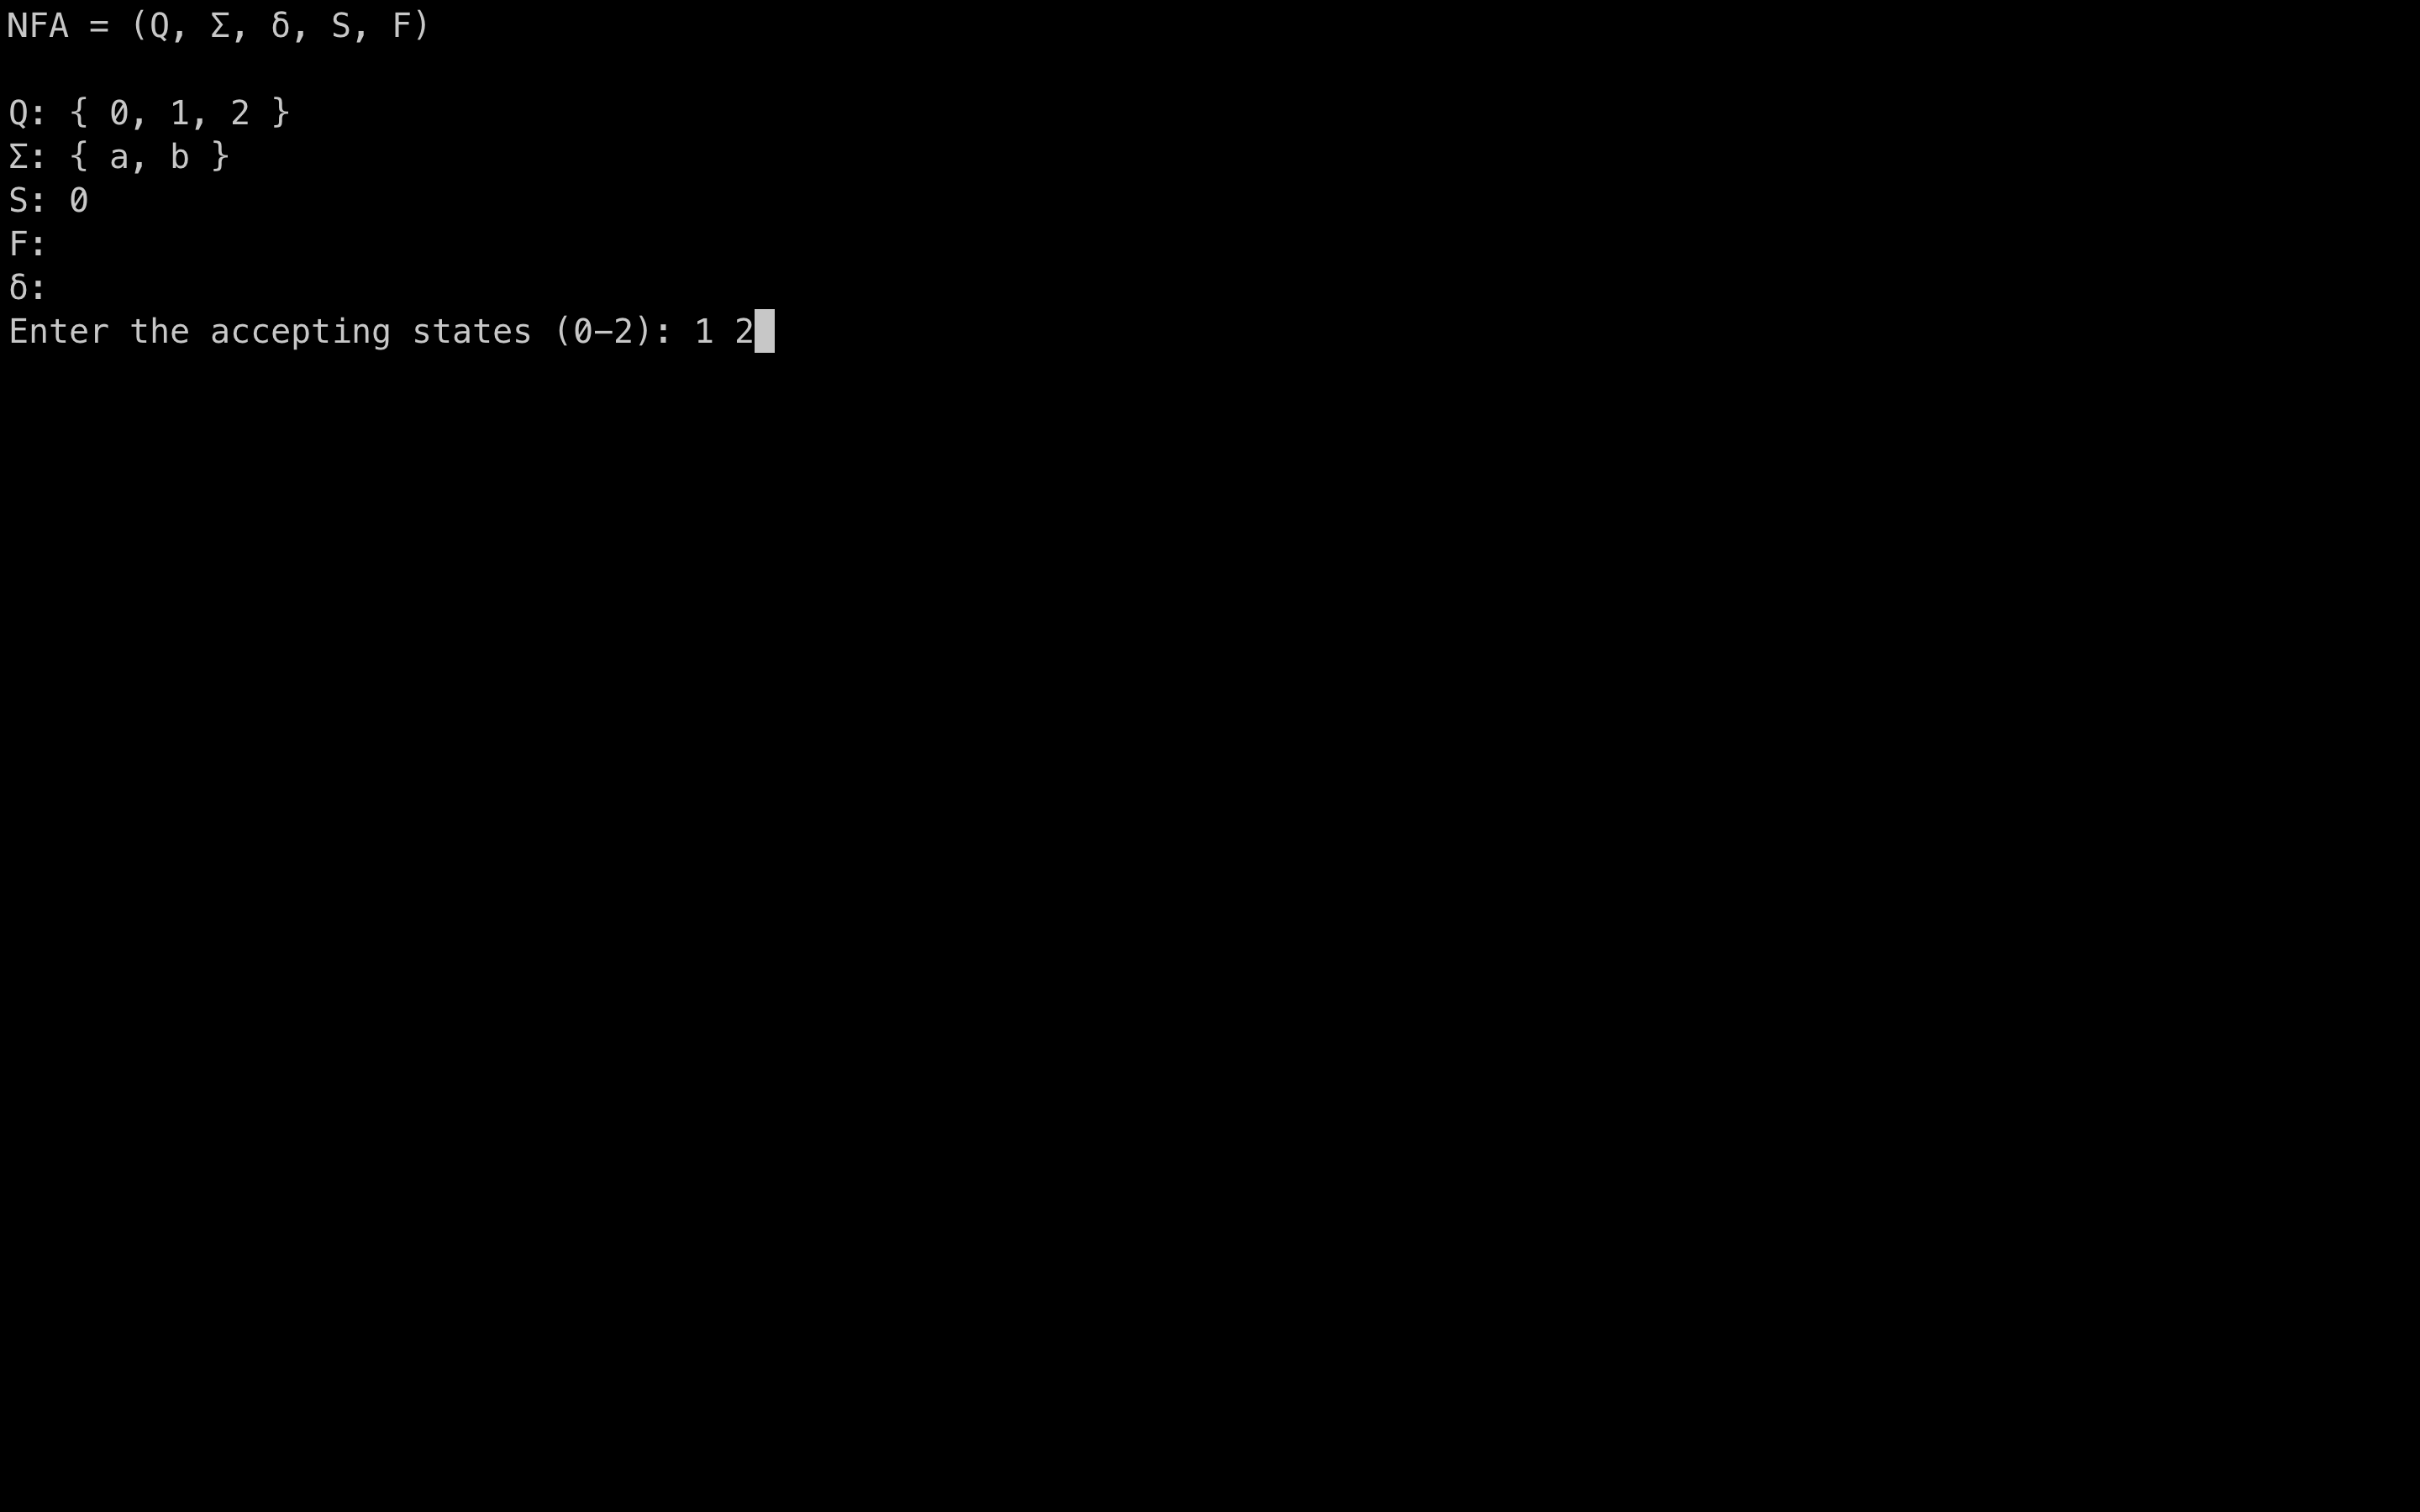
\includegraphics[width=0.8\textwidth]{accept}
\end{center}

\textbf{\large Enter the corresponding output}

When entering the outputs of the transition function for the $N$, the program sequentially prompts for the output corresponding to each state and input symbol pair. For example, we are prompted for the output corresponding to the pair $(0, a)$ in the image, considering the transition function of $N$ maps state 0 with input symbol $a$ to the set $\{1\}$, we input \verb|1|.

\begin{center}
  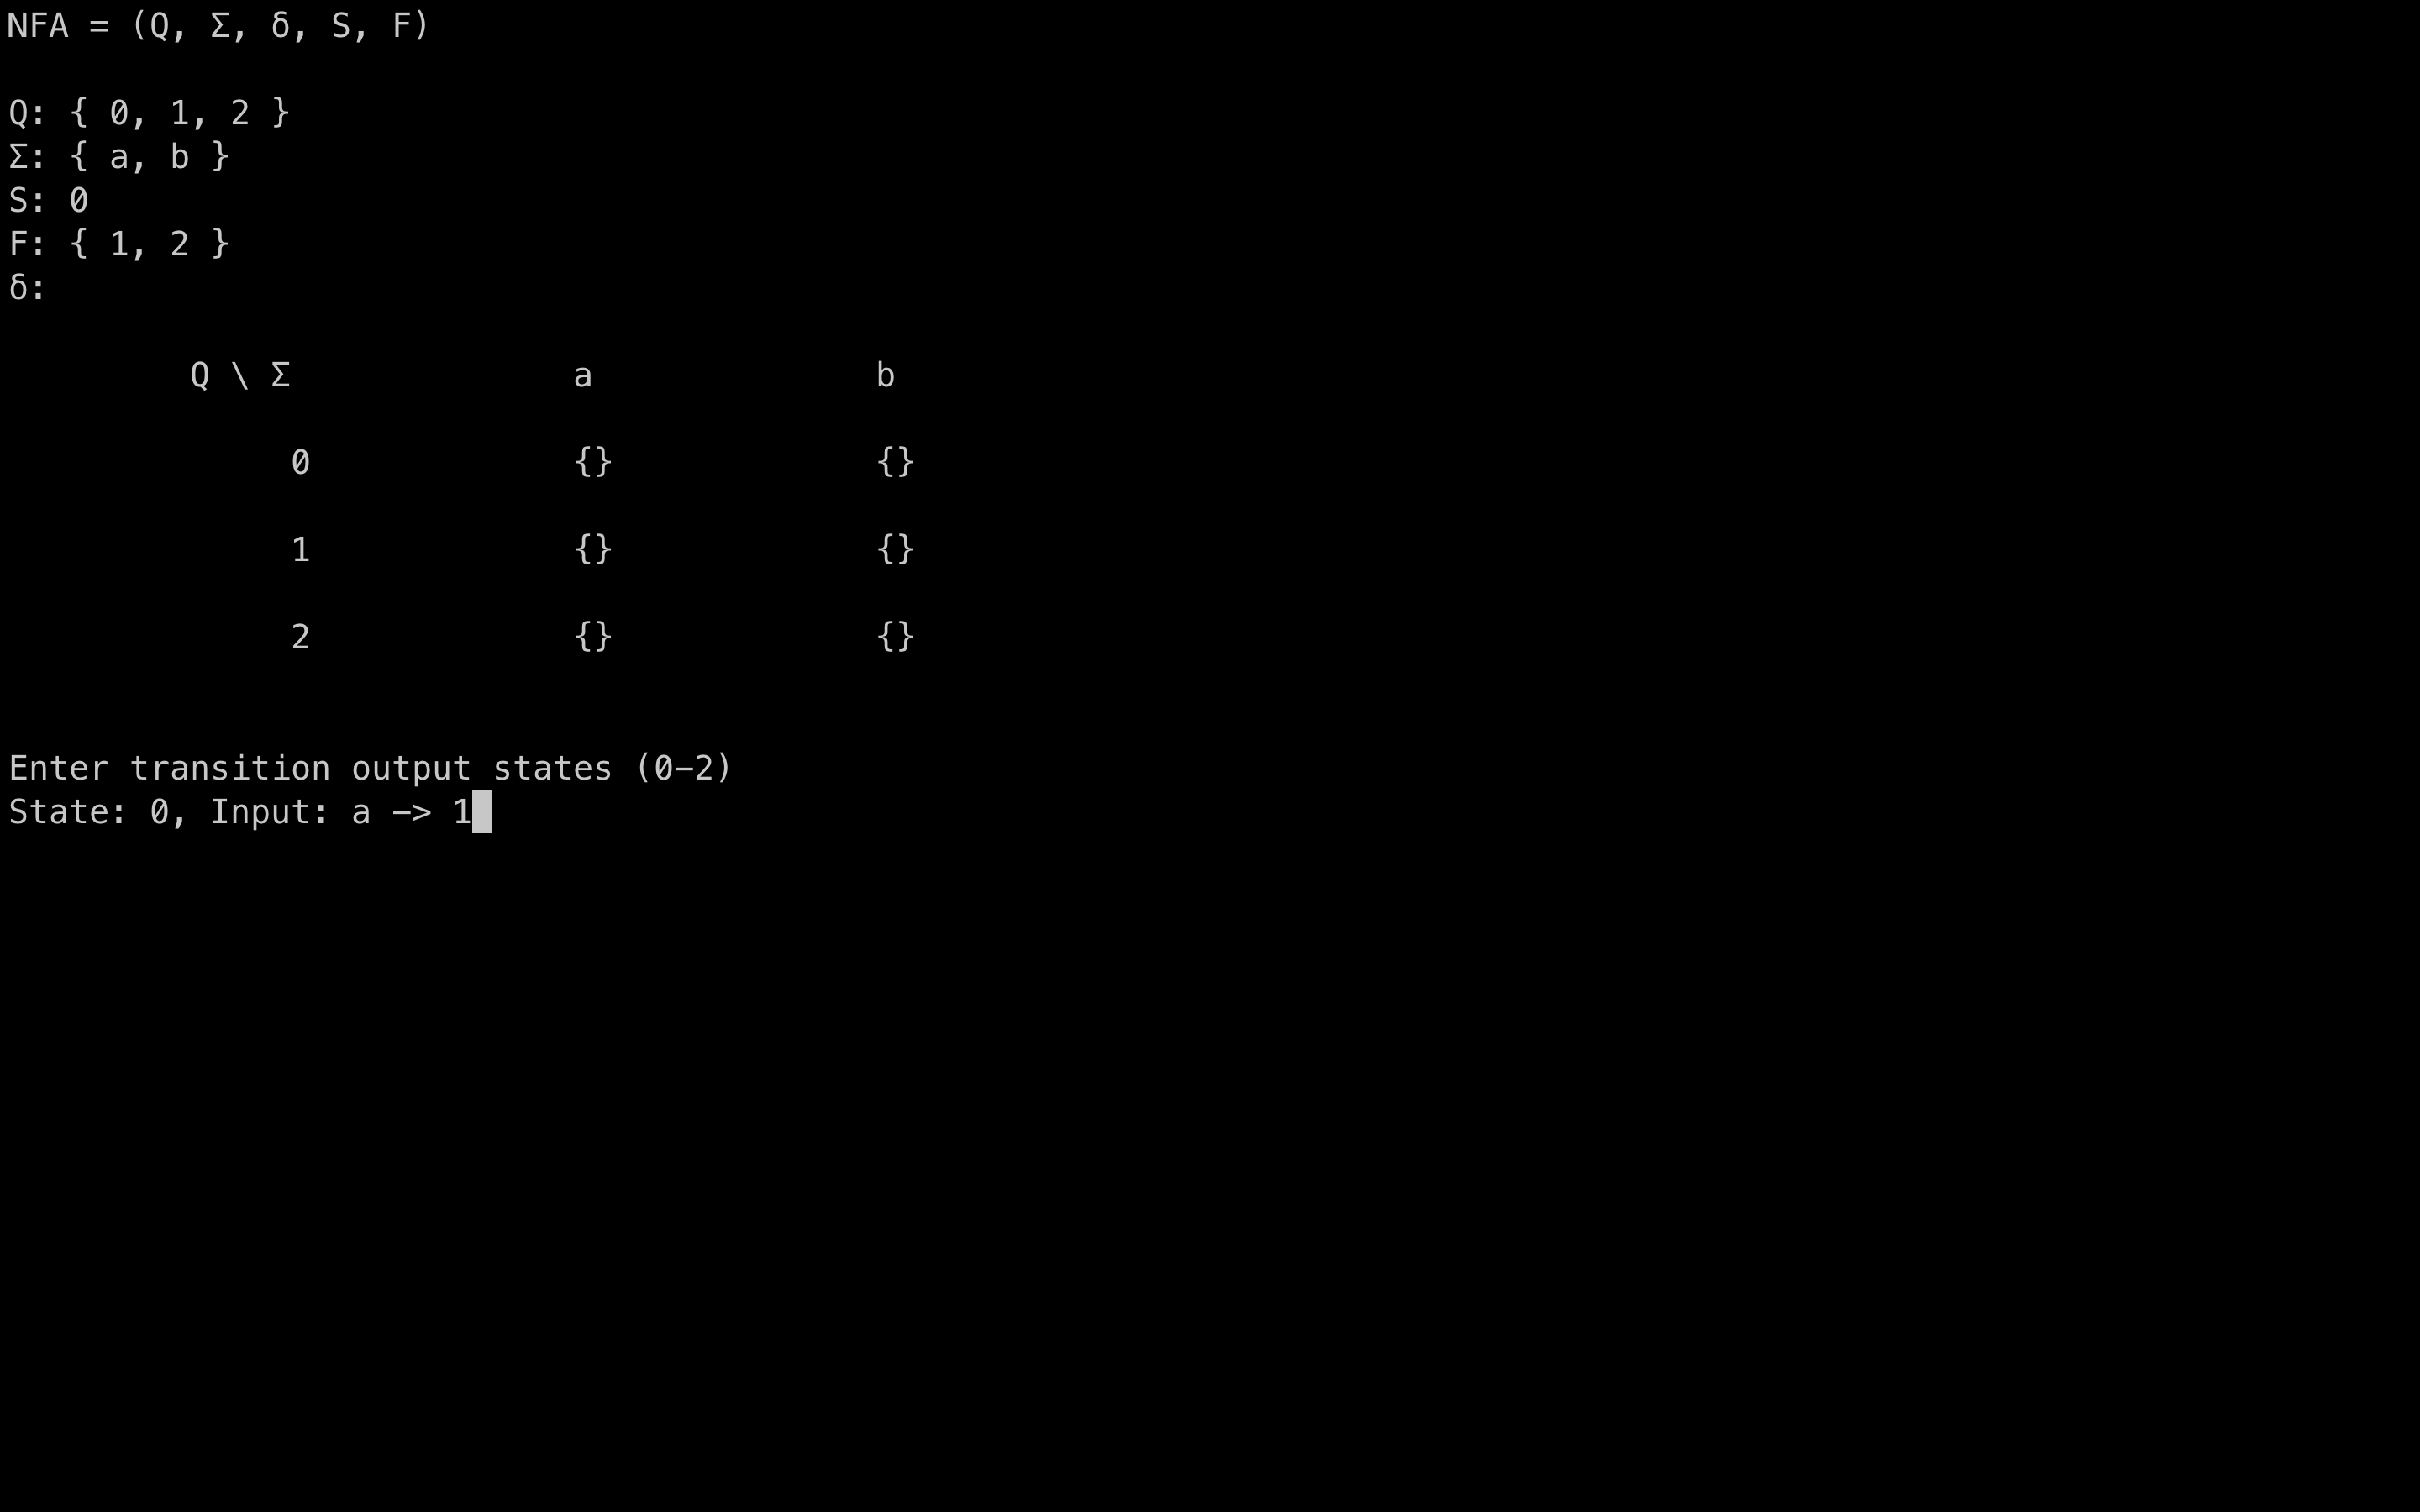
\includegraphics[width=0.8\textwidth]{trans}
\end{center}

\newpage

\section*{Result}

After completing the input process, the program will display the formal definition of $N$ alongside the converted DFA derived from $N$.

\begin{center}
  \begin{multicols}{2}
    Representation of $N$

    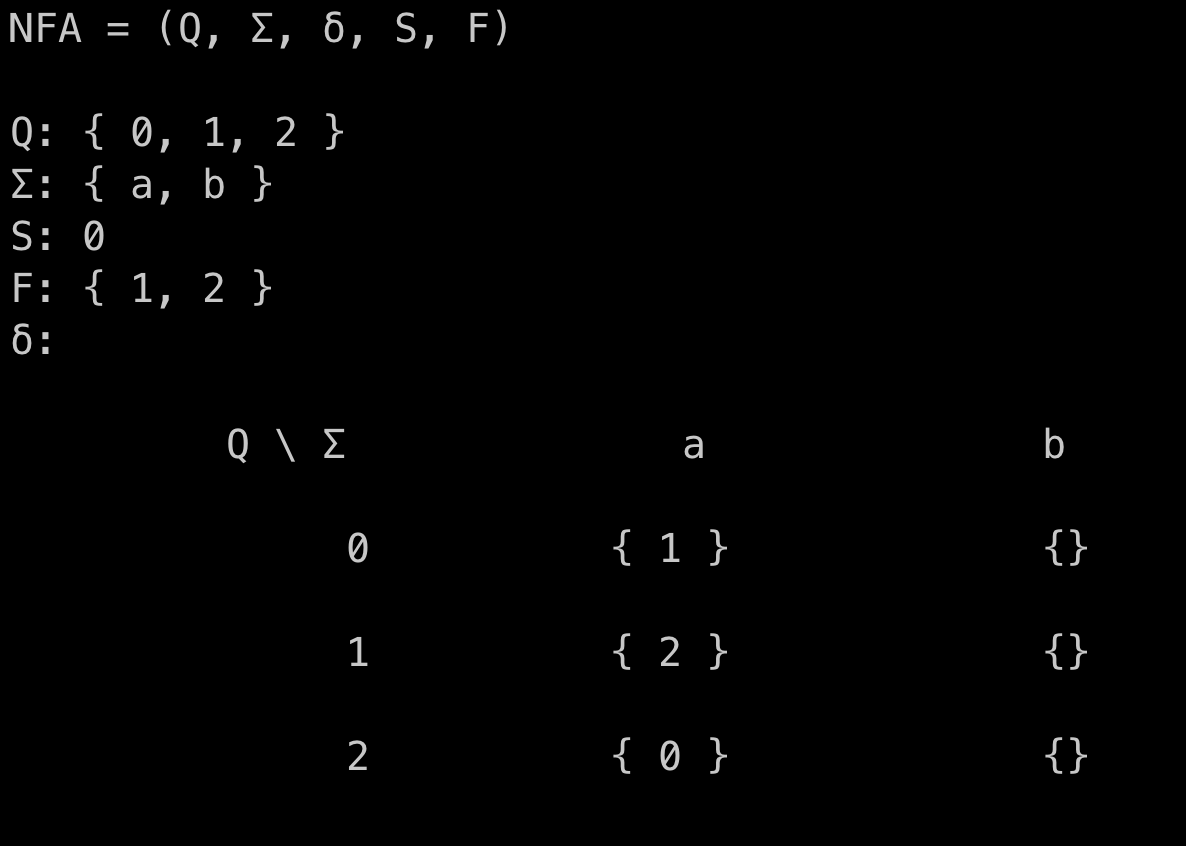
\includegraphics[width=0.45\textwidth]{NFA}

    \columnbreak 

    Resulting DFA $N'$

    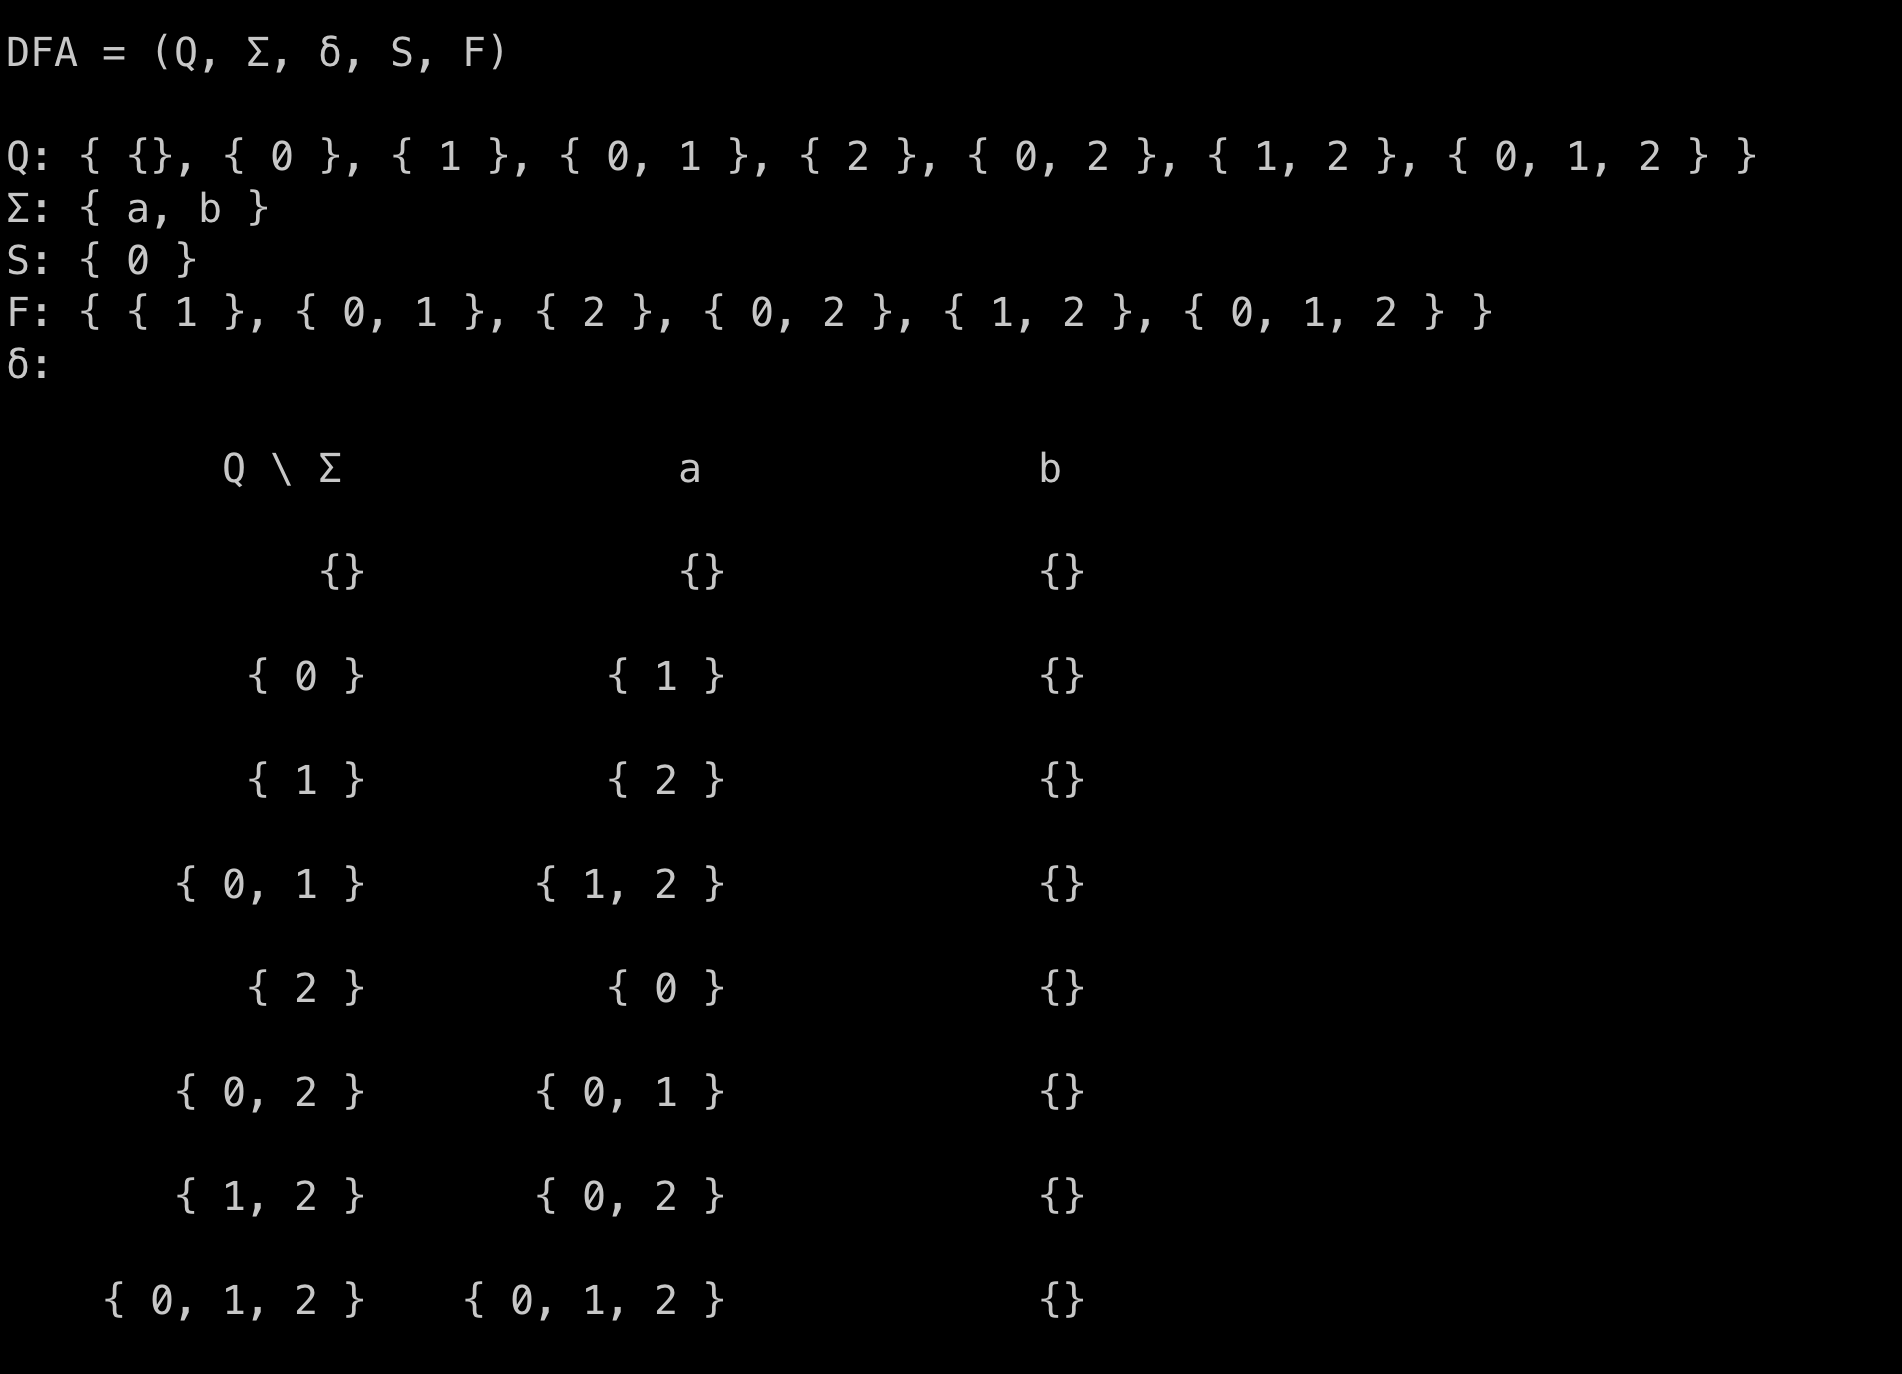
\includegraphics[width=0.45\textwidth]{DFA}
  \end{multicols}
\end{center}

Call that resulting DFA $N'$. We now confirm that $N'$ recognizes the same language as $N$. Suppose $w \in L(N)$. Say $w = \underbrace{aa \dots a}_{k}$, for some $k \nmid 3$. Notice that when the input string only contains $a$, $N'$ would cycle through the states $\{0\} \rightarrow \{1\} \rightarrow \{2\} \rightarrow \{0\}$. Since $\{0\}$ is both the starting state of $N'$ and the only non-accepting states in the cycle, $w$ will be accepted by $N'$, as it has length not divisible by 3 so it would not end at $\{0\}$. We now suppose $w \notin L(N)$. If $w$ contains $b$, it would get immediately sent to $\{\}$, whose only output state is itself, so $w$ would get stuck in $\{\}$ and never reach an accepting state. Hence, we may assume $w$ does not contain $b$. Then, $w$ contains only $a$'s and is of length divisible by $3$. As shown above, $w$ will stay in the cycle $\{0\} \rightarrow \{1\} \rightarrow \{2\} \rightarrow \{0\}$, but this time $w$ must end up at $\{0\}$, so it would get
rejected by $N'$. Therefore, $L(N) = L(N')$, so the output for this example is indeed correct.

\pagebreak

\section*{Code}

\subsection*{Makefile}

\begin{lstlisting}
CXX = clang++
CXXFLAGS = -Wall -pedantic -g -O0 -std=c++11
TARGET = convert
OBJ = main.o NFA.o DFA.o

all: $(TARGET)

$(TARGET): $(OBJ)
	$(CXX) $(CXXFLAGS) -o $(TARGET) $(OBJ)

main.o: main.cpp NFA.h DFA.h
	$(CXX) $(CXXFLAGS) -c main.cpp

NFA.o: NFA.cpp NFA.h
	$(CXX) $(CXXFLAGS) -c NFA.cpp

DFA.o: DFA.cpp DFA.h
	$(CXX) $(CXXFLAGS) -c DFA.cpp

clean:
	rm -f $(TARGET) $(OBJ)
\end{lstlisting}

\subsection*{main.cpp}

\begin{lstlisting}[language=C++]
#include <iostream> #include "NFA.h" #include "DFA.h" using namespace std;

int main() { NFA nfa = NFA();

	nfa.init();

	cout << endl;

	DFA* dfa = nfa.convert(); dfa->display();

	return 0; }
\end{lstlisting}

\newpage

\subsection*{NFA.h}

\begin{lstlisting}[language=C++]
#ifndef NFA_H #define NFA_H

#include "DFA.h" #include <iostream> #include <cstdlib> #include <vector> #include <string> #include <sstream> #include <iomanip> using namespace std;

class NFA {

  int states; vector<char> sigma; vector<vector<int>> delta; int start; int accept;

  public:

    NFA();

    void init();

    void inputStates();

    void inputStart();

    void inputAccept();

    void inputDelta();

    string bin2set(int bin);

    void printTable();

    DFA* convert();
    
    void display(); };

#endif
\end{lstlisting}

\newpage

\subsection*{NFA.cpp}

\begin{lstlisting}
#include "NFA.h"
using namespace std;

NFA::NFA(): states(0), sigma{'a', 'b'}, start(-1), accept(0) {}

void NFA::init() {
  display();
  inputStates();
  inputStart();
  inputAccept();
  inputDelta();
  display();
}

void NFA::inputStates() {
  cout << "Enter the number of states: ";
  cin >> states;
  delta = vector<vector<int>>(states, vector<int>(2, 0));
  display();
}

void NFA::inputStart() {
  cout << "Enter the starting state (0-" << states - 1 << "): ";
  cin >> start;
  display();
}

void NFA::inputAccept() {
  cin.ignore(numeric_limits<streamsize>::max(), '\n');

  cout << "Enter the accepting states (0-" << states - 1 << "): ";
  string line;
  getline(cin, line);
  istringstream iss(line);
  int acceptState;
  while (iss >> acceptState)
    accept |= (1 << acceptState);
  display();
}

void NFA::inputDelta() {
  for (int s = 0; s < states; s++) {
    for (int a = 0; a < sigma.size(); a++) {
      cout << "Enter transition output states (0-" << states - 1 << ")" << endl;
      cout << "State: " << s << ", Input: " << sigma[a] << " -> ";
      string line;
      getline(cin, line);
      istringstream iss(line);
      int outState;
      while (iss >> outState)
        delta[s][a] |= (1 << outState);
      display();
    }
  }
}

string NFA::bin2set(int bin) {
  if (bin == 0) return "{}";
  string str = "{ ";
  int cnt = 0;
  bool first = true;
  while (bin > 0) {
    if (bin & 1) {
      if (!first)
        str += ", ";
      str += to_string(cnt);
      first = false;
    }
    bin >>= 1;
    cnt++;
  }
  str += " }";
  return str;
}

DFA* NFA::convert() {
  return new DFA(states, sigma, delta, start, accept);
}

void NFA::printTable() {
  int width = 15;
  cout << setw(width) << "Q \\ \u03A3";
  for (char a : sigma)
    cout << setw(width) << a;
  cout << "\n\n";

  for (int state = 0; state < states; state++) {
    cout << setw(width) << state;
    for (int sig = 0; sig < sigma.size(); sig++) {
      ostringstream cell;
      cell << bin2set(delta[state][sig]);
      cout << setw(width) << cell.str();
    }
    cout << "\n\n";
  }
}

void NFA::display() {
  system("clear");
  cout << "NFA = (Q, \u03A3, \u03B4, S, F)" << "\n\n";

  cout << "Q: ";
  if (states) {
    cout << "{ ";
    for (int i = 0; i < states - 1; i++) {
      cout << i << ", ";
    }
    cout << states - 1 << " }";
  }
  cout << endl;

  cout << "\u03A3: ";
  if (!sigma.empty()) {
    cout << "{ ";
    for (int i = 0; i < sigma.size() - 1; i++) {
      cout << sigma[i] << ", ";
    }
    cout << sigma[sigma.size() - 1] << " }";
  }
  cout << endl;

  cout << "S: ";
  if (start > -1)
    cout << start;
  cout << endl;

  cout << "F: ";
  if (accept)
    cout << bin2set(accept);
  cout << endl;

  cout << "\u03B4: ";
  if (accept) {
    cout << "\n\n";
    printTable();
  }
  cout << endl;
}
\end{lstlisting}

\newpage

\subsection*{DFA.h}

\begin{lstlisting}
#ifndef DFA_H
#define DFA_H

#include <vector>
#include <string>
#include <iostream>
#include <sstream>
#include <iomanip>
using namespace std;

class DFA {
    
	int states;
	vector<char> sigma;
	vector<vector<int>> delta;
	int start;
	int accept;

	public:

		DFA(int NFAstates, vector<char>& NFAsigma, vector<vector<int>>& NFAdelta, int NFAstart, int NFAaccept);

		void init();

		string bin2set(int bin);

		void printTable();

		void display();
};

#endif
\end{lstlisting}

\newpage

\subsection*{DFA.cpp}

\begin{lstlisting}
#include "DFA.h"
using namespace std;

DFA::DFA(int NFAstates, vector<char>& NFAsigma, vector<vector<int>>& NFAdelta, int NFAstart, int NFAaccept): start(NFAstart), accept(NFAaccept) {
  states = 1 << NFAstates;
  sigma = NFAsigma;
  delta = vector<vector<int>>(states, vector<int>(2, 0));
  for (int s = 0; s < states; s++) {
    for (int a = 0; a < sigma.size(); a++) {
      int temp = s;
      int cnt = 0;
      while (temp > 0) {
        if (temp & 1)
          delta[s][a] |= NFAdelta[cnt][a];
        cnt++;
        temp >>= 1;
      }
    }
  }
};

string DFA::bin2set(int bin) {
  if (bin == 0) return "{}";
  string str = "{ ";
  int cnt = 0;
  bool first = true;
  while (bin > 0) {
    if (bin & 1) {
      if (!first)
        str += ", ";
      str += to_string(cnt);
      first = false;
    }
    bin >>= 1;
    cnt++;
  }
  str += " }";
  return str;
}

void DFA::printTable() {
  int width = 15;
  cout << setw(width) << "Q \\ \u03A3";
  for (char a : sigma) {
    cout << setw(width) << a;
  }
  cout << "\n\n";

  for (int s = 0; s < states; s++) {
    ostringstream cell;
    cell << bin2set(s);
    cout << setw(width) << cell.str();

    for (int a = 0; a < sigma.size(); a++) {
      ostringstream cell;
      cell << bin2set(delta[s][a]);
      cout << setw(width) << cell.str();
    }
    cout << "\n\n";
  }
};

void DFA::display() {
  cout << "DFA = (Q, \u03A3, \u03B4, S, F)" << "\n\n";

  cout << "Q: { ";
  for (int i = 0; i < states - 1; i++)
    cout << bin2set(i) << ", ";
  cout << bin2set(states - 1) << " }" << endl;

  cout << "\u03A3: { ";
  for (int i = 0; i < sigma.size() - 1; i++)
    cout << sigma[i] << ", ";
  cout << sigma[sigma.size() - 1] << " }" << endl;

  cout << "S: { " << start << " }" << endl;

  cout << "F: { ";
  bool first = false;
  for (int i = 0; i < states; i++) {
    if (i & accept) {
      if (first)
        cout << ", ";
      first = true;
      cout << bin2set(i);
    }
  }
  cout << " }" << endl;

  cout << "\u03B4: ";
  cout << "\n\n";
  printTable();
  cout << endl;
};
\end{lstlisting}

\end{document}